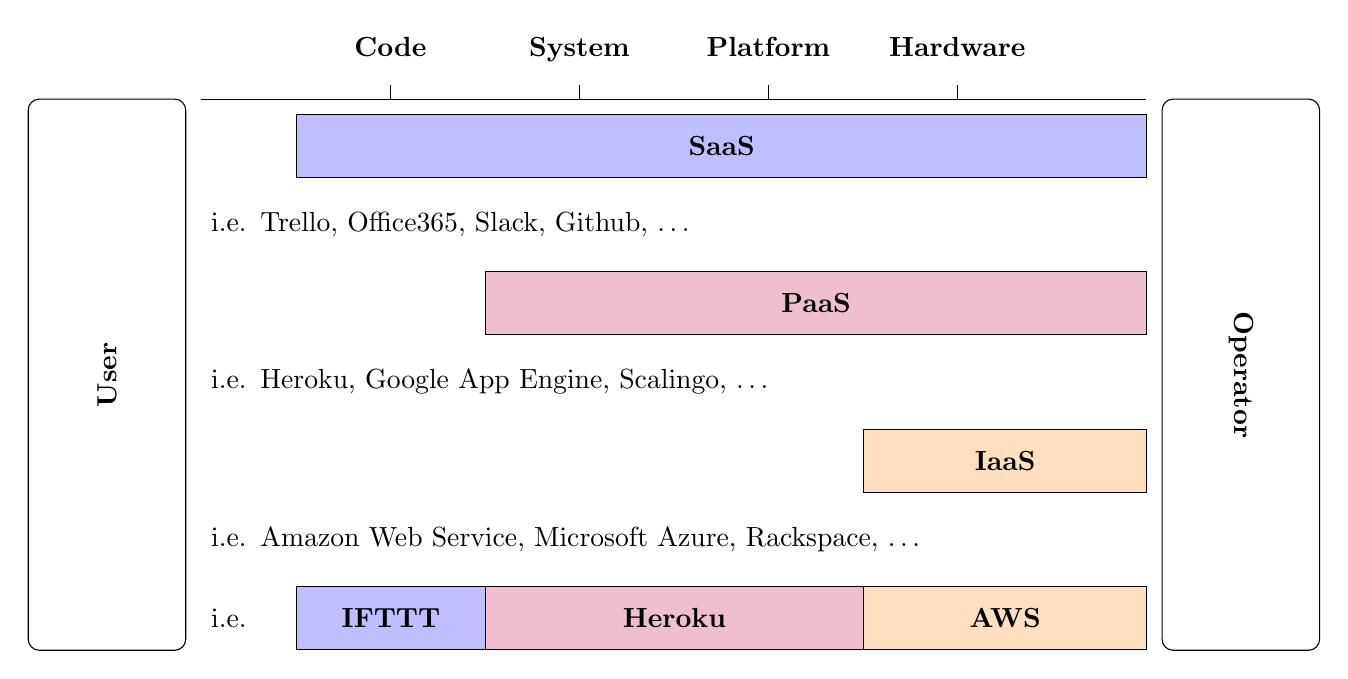
\begin{tikzpicture}[x=12mm,y=10mm,
every node/.style={font=\bfseries},
bar/.style={%
draw,
anchor=south west,
minimum height=8mm
},
party/.style={%
draw,
minimum width=70mm,
rounded corners,
anchor=center,
minimum height=20mm
},
ex/.style={%
font=\mdseries,
anchor=south west,
align=left,
text width=120mm,
minimum height=8mm
}]
\draw[] (0,0) -- (10,0);
\node[party,rotate=90]at(-1,-3.5){User};
\node[party,rotate=-90]at(11,-3.5){Operator};
\foreach \n[count=\i from 1] in {Code\\,System\\,Platform\\,Hardware\\}{%
\draw (\i*2,5pt)--(\i*2,0pt) node[anchor=south,align=center]{\n};
}
\node[bar,minimum width=108mm,fill=blue!25]at(1,-1){SaaS};
\node[ex]at(0,-2){i.e. Trello, Office365, Slack, Github, \ldots};
\node[bar,minimum width=84mm,fill=purple!25]at(3,-3){PaaS};
\node[ex]at(0,-4){i.e. Heroku, Google App Engine, Scalingo, \ldots};
\node[bar,minimum width=36mm,fill=orange!25]at(7,-5){IaaS};
\node[ex]at(0,-6){i.e. Amazon Web Service, Microsoft Azure, Rackspace, \ldots};
\node[ex,minimum width=10mm]at(0,-7){i.e.};
\node[bar,minimum width=24mm,fill=blue!25]at(1,-7){IFTTT};
\node[bar,minimum width=48mm,fill=purple!25]at(3,-7){Heroku};
\node[bar,minimum width=36mm,fill=orange!25]at(7,-7){AWS};
\end{tikzpicture}
